\documentclass[a4paper,11pt]{article}

\usepackage[empty]{fullpage}
\usepackage{titlesec}
\usepackage[usenames,dvipsnames]{color}
\usepackage{enumitem}
\usepackage{fancyhdr}
\usepackage[english]{babel}
\usepackage{tabularx}
\usepackage{fontawesome5}
\usepackage{multicol}
\usepackage{graphicx}
\usepackage[export]{adjustbox}
\usepackage[sfdefault]{roboto}
\usepackage[hidelinks]{hyperref}
\usepackage{montserrat}


\setlength{\multicolsep}{3.0pt}
\setlength{\columnsep}{5pt}

% Adjust footer
\pagestyle{fancy}
\fancyhf{} % clear all header and footer fields
\renewcommand{\headrulewidth}{0pt}
\renewcommand{\footrulewidth}{0pt}
\setlength{\footskip}{5pt} % Increase footskip to resolve fancyhdr warning

% Adjust margins
\addtolength{\oddsidemargin}{-0.5in}
\addtolength{\evensidemargin}{-0.5in}
\addtolength{\textwidth}{1.0in}
\addtolength{\topmargin}{-.7in}
\addtolength{\textheight}{1.3in}

\urlstyle{same}

\raggedbottom
\raggedright
\setlength{\tabcolsep}{0in}

% Sections formatting
\titleformat{\section}{
	\vspace{-6pt}\scshape\raggedright\large\bfseries
}{}{0em}{}[\color{black}\titlerule \vspace{-7pt}]

% Ensure that generate pdf is machine readable/ATS parsable
\pdfgentounicode=1

% Custom commands
\newcommand{\resumeItem}[1]{
	\item\small{#1 \vspace{-2pt}}
}

\newcommand{\resumeSubheading}[4]{
	\vspace{-2pt}\item
		\begin{tabular*}{0.97\textwidth}[t]{l@{\extracolsep{\fill}}r}
			\textbf{#1} & \textbf{\small #2} \\
			\textit{\small#3} & \textit{\small #4} \\
		\end{tabular*}\vspace{-7pt}
}

\newcommand{\resumeProjectHeading}[2]{
		\item
		\begin{tabular*}{0.97\textwidth}{l@{\extracolsep{\fill}}r}
			\small#1 & \textbf{\small #2} \\
		\end{tabular*}\vspace{-7pt}
}

\newcommand{\resumeSubHeadingListStart}{\begin{itemize}[leftmargin=0.15in, label={}]}
\newcommand{\resumeSubHeadingListEnd}{\end{itemize}}
\newcommand{\resumeItemListStart}{\begin{itemize}}
\newcommand{\resumeItemListEnd}{\end{itemize}\vspace{-5pt}}

\begin{document}

\begin{minipage}[c]{0.15\textwidth}
	\fbox{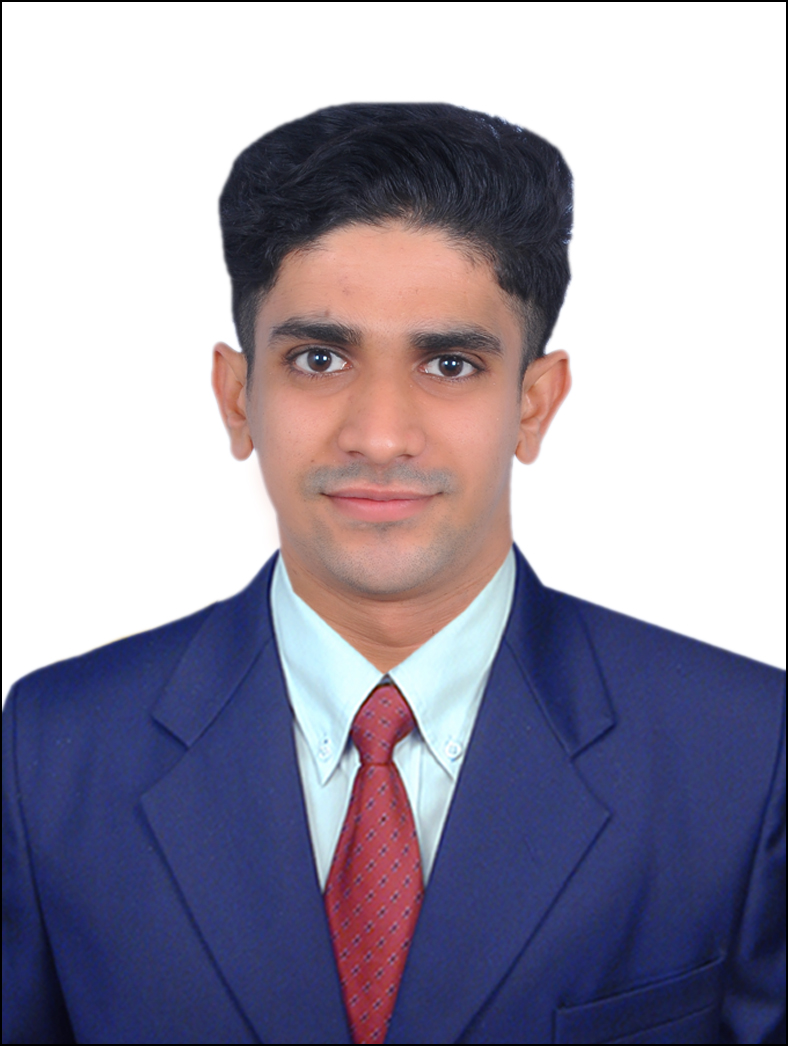
\includegraphics[width=0.84\textwidth]{photo.jpg}}
\end{minipage}
\begin{minipage}[t]{0.84\textwidth}  % Adjusted width to fill space
	\begin{center}
		{\fontfamily{Montserrat-TOsF}\selectfont \textbf{\Huge \scshape {Fahim Firoz Fadi}}} \\ \vspace{1pt}
		\small{
			\raisebox{-0.1\height}\faPhone\ \href{tel:+917736634869}{\underline{+91 7736634869}} $|$
			\raisebox{-0.2\height}\faEnvelope\ \href{mailto:fahimfadi2021@gmail.com}{\underline{fahimfadi2021@gmail.com}} $|$
			\raisebox{-0.2\height}\faLinkedin\ \href{https://www.linkedin.com/in/fahim-fadi-816155310}{\underline{linkedin.com/fahim-fadi}}
		}
	\end{center}
\end{minipage}


\section{Summary}
\begin{itemize}[leftmargin=0.15in, label={}]
	\small{\item{
		Enthusiastic and customer-focused individual with a passion for providing exceptional in-flight service and ensuring passenger safety. Trained in cabin crew responsibilities including safety procedures, emergency protocols, and customer service. Possesses excellent communication skills, a calm and professional demeanor, and a strong ability to work in a team-oriented and fast-paced environment. Dedicated to creating a comfortable and positive experience for passengers while upholding the highest standards of hospitality and safety.
				}}
\end{itemize}
\section{Education}
\resumeSubHeadingListStart
\resumeSubheading
{Krupanidhi Degree College}{Bengaluru, Karnataka}
{Bachelor of Computer Applications}{Aug. 2021 -- Sep. 2024}
\resumeSubheading
{Al Ameen PU College}{Bengaluru, Karnataka}
{Science}{June 2019 -- March 2021}
%  \resumeSubheading {International Indian School Dammam}{Dammam, Saudi Arabia}{CBSE}{March 2017}
\resumeSubHeadingListEnd

%\section{Relevant Coursework}
%\begin{itemize}[leftmargin=*,nosep]
%  \begin{multicols}{4}
%    \item Computer Networks
%    \item Operating Systems
%    \item Database Management% Systems
%    \item Web Development
%    \item Data Structures% and Algorithms
%    \item Cyber Security
%    \item Software Engineering
%    \item Cloud Computing
%  \end{multicols}
%\end{itemize}

% \section{Core Competencies}
% \begin{itemize}[leftmargin=*,nosep]
% 	\begin{multicols}{3}
% 		\item Full Stack Development
% 		\item System Optimization 
% 		\item API Development
% 		\item Cloud Deployment
% 		\item Troubleshooting and Debugging
% 		\item Quality Assurance and Testing
% 	\end{multicols}
% \end{itemize}

\section{Experience}
\resumeSubHeadingListStart
\resumeSubheading
{Dominos Pizza}{May 2022 -- March 2025}
{Customer Service Representative}{Bengaluru, Karnataka}
\resumeItemListStart
\resumeItem{Delivered exceptional customer service, handling in-person and phone orders with professionalism and accuracy in a fast-paced environment.}
\resumeItem{\textbf{Order Management:} Processed and tracked hundreds of daily orders using proprietary POS systems, ensuring smooth workflow and timely delivery.}
\resumeItem{\textbf{Conflict Resolution:} Addressed and resolved customer concerns effectively, consistently maintaining satisfaction scores above company benchmarks.}
\resumeItem{\textbf{Team Collaboration \& Support:} Coordinated with kitchen staff and delivery partners to streamline operations and avoid service delays.}
\resumeItem{\textbf{Operational Contribution:} Maintained store cleanliness, restocked inventory, and supported training of new staff to enhance overall team performance.}
\resumeItemListEnd
% \resumeSubheading
% {ETAYA INNOVATIONS Pvt Ltd}{Nov 2024 -- Present}
% {Flutter Developer Intern}{Bengaluru, Karnataka}
% \resumeItemListStart
% \resumeItem{Working as a full-time Flutter developer at \textbf{ETAYA INNOVATIONS Pvt Ltd}, developing and maintaining cross-platform mobile applications for Android and iOS using Flutter and Dart.}
% \resumeItem{\textbf{Flutter App Development:} Designed and built scalable, high-performance mobile applications, implementing clean architecture, provider-based state management, and custom UI components.}
% \resumeItem{\textbf{Backend Integration and API Handling:} Integrated RESTful APIs and Firebase services for real-time data synchronization, authentication, push notifications, and secure cloud storage.}
% \resumeItem{\textbf{Performance Optimization:} Improved app efficiency by optimizing widget rebuilds, implementing lazy loading, and reducing API call overhead, resulting in smoother UI interactions and faster load times.}
% \resumeItem{\textbf{Testing and Debugging:} Conducted automated and manual testing using Flutter’s testing framework and Firebase Crashlytics to identify and resolve UI inconsistencies, crashes, and performance bottlenecks.}
% \resumeItem{\textbf{Agile Development and Collaboration:} Worked in an Agile environment, participating in sprint planning, peer code reviews, and cross-functional team collaborations to deliver feature-rich applications on time.}
% \resumeItemListEnd
\resumeSubHeadingListEnd

% \section{Projects}
% \resumeSubHeadingListStart
% \resumeProjectHeading
% {\textbf{\href{https://github.com/ajmalbuv/EduManage}{\underline{EduManage}}} $|$ \emph{Python, Django, PostgreSQL, Docker}}{July 2024}
% \resumeItemListStart
% \resumeItem{\textbf{Developed and Deployed Scalable Web Application:} Built an end-to-end web application using Django and PostgreSQL, enhancing data management and administrative efficiency for users.}
% \resumeItem{\textbf{Cross-Platform Deployment for High Availability:} Implemented on an Ubuntu VPS with Gunicorn and Certbot for SSL, as well as Vercel using serverless functions, ensuring 99\%+ uptime.}
% \resumeItem{\textbf{Optimized Database and Security:} Designed efficient database schemas and deployed SSL encryption to secure user data, achieving a 30\% improvement in query performance.}
% \resumeItem{\textbf{Collaborative Version Control:} Leveraged GitHub for collaborative development, enhancing workflow efficiency and documentation for seamless project management.}
% \resumeItemListEnd
% \resumeSubHeadingListEnd

% \section{Technical Skills}
% \begin{itemize}[leftmargin=0.15in, label={}]
% 	\small{\item{
% 				\textbf{Programming Languages}{: Python, Java, JavaScript, SQL, C, PHP, Dart, R}\\
% 				\textbf{Web Technologies}{: HTML5, CSS3, React.js, Node.js, Django, Flask, REST APIs, Flutter}\\
% 				\textbf{Databases \& Tools}{: PostgreSQL, MongoDB, Docker (containers), Git (version control), Oracle Cloud}\\
% 				\textbf{Development Tools}{: VS Code, PyCharm, IntelliJ, Postman, Android Studio, Vercel}
% 				}}
% \end{itemize}


\section{Skills \& Competencies}
\begin{itemize}[leftmargin=0.15in, label={}, itemsep=0pt]
	\small{
		\item \textbf{Customer Service}: Professional communication, conflict resolution, guest satisfaction, complaint handling
		\item \textbf{Safety \& Emergency Response}: Basic first aid, safety protocols, evacuation assistance, calm crisis management
		\item \textbf{Communication Skills}: Clear verbal interaction, multilingual abilities, active listening, tone modulation
		\item \textbf{Teamwork \& Collaboration}: Crew coordination, cross-functional support, shift teamwork, task sharing
		\item \textbf{Presentation \& Grooming}: Uniform standards, personal hygiene, posture control, brand representation
		\item \textbf{Adaptability \& Professionalism}: Quick learning, cultural sensitivity, punctuality, rule adherence
	}
\end{itemize}

\section{Languages}
\begin{itemize}[leftmargin=0.15in, label={}]
    \small{\item{
                \textbf{English   }{- Fluent}\\
                \textbf{Hindi     }{- Fluent}\\
                \textbf{Arabic    }{- Conversational}\\
                \textbf{Malayalam }{- Native Speaker}\\
                \textbf{Tamil     }{- Fluent}\\
                \textbf{Kannada   }{- Fluent}\\
                \textbf{Telugu    }{- Conversational}\\
                \textbf{Urdu      }{- Fluent}
                }}
\end{itemize}

\end{document}
